% it consist of grid-related electricity metrics.
% Other purpose, the fact that they have the 'same' client [although I think they are different research groups], and the differences,
\section{Monitor electricity consumption}
As the section title states, here we propose a possible approach to monitor the energy consumption of a large campus, the \ac{BHC} in Belgium using existing information, that have been collected over several years.
We also outlined some of the practical difficulties encountered in ingesting, analysing, and visualising the data, 
where understanding the underlying context of the project proved to be an important dimension. 
It is therefore relevant to bear in mind that this is a university-oriented project, therefore pragmatic and data-oriented rather than presentation-oriented.
Despite all difficulties, the product is currently up and running, with new data sources on the way.

\subsection{Initial Hypothesis}\label{sub:vub_initial_hp}
\paragraph{Client} 
% with the motto: \textit{"Conquering darkness by science"} 
\ac{GEP} is a joint project of the \ac{VUB} (Free University of Brussels), dutch and English-speaking research university, and the \ac{UZB} (University Hospital of Brussels), 
whose purpose is to develop and operate a research campus in the Research Park of Zellik with a focus on the following three research domains:
\begin{itemize}
    \item Energy and mobility transition.
    \item Hospital of the future, part of \ac{BHC}.
    \item Smart regions.
\end{itemize}
With this research campus, Green Energy Park aims at bridging the gap between research, innovation, realization and exploitation, by acting as a large-scale living lab, expertise and training centre~\cite{Misc:vub_2020_green}.
\paragraph{Context Introduction}
\begin{figure}[ht]
    \fbox{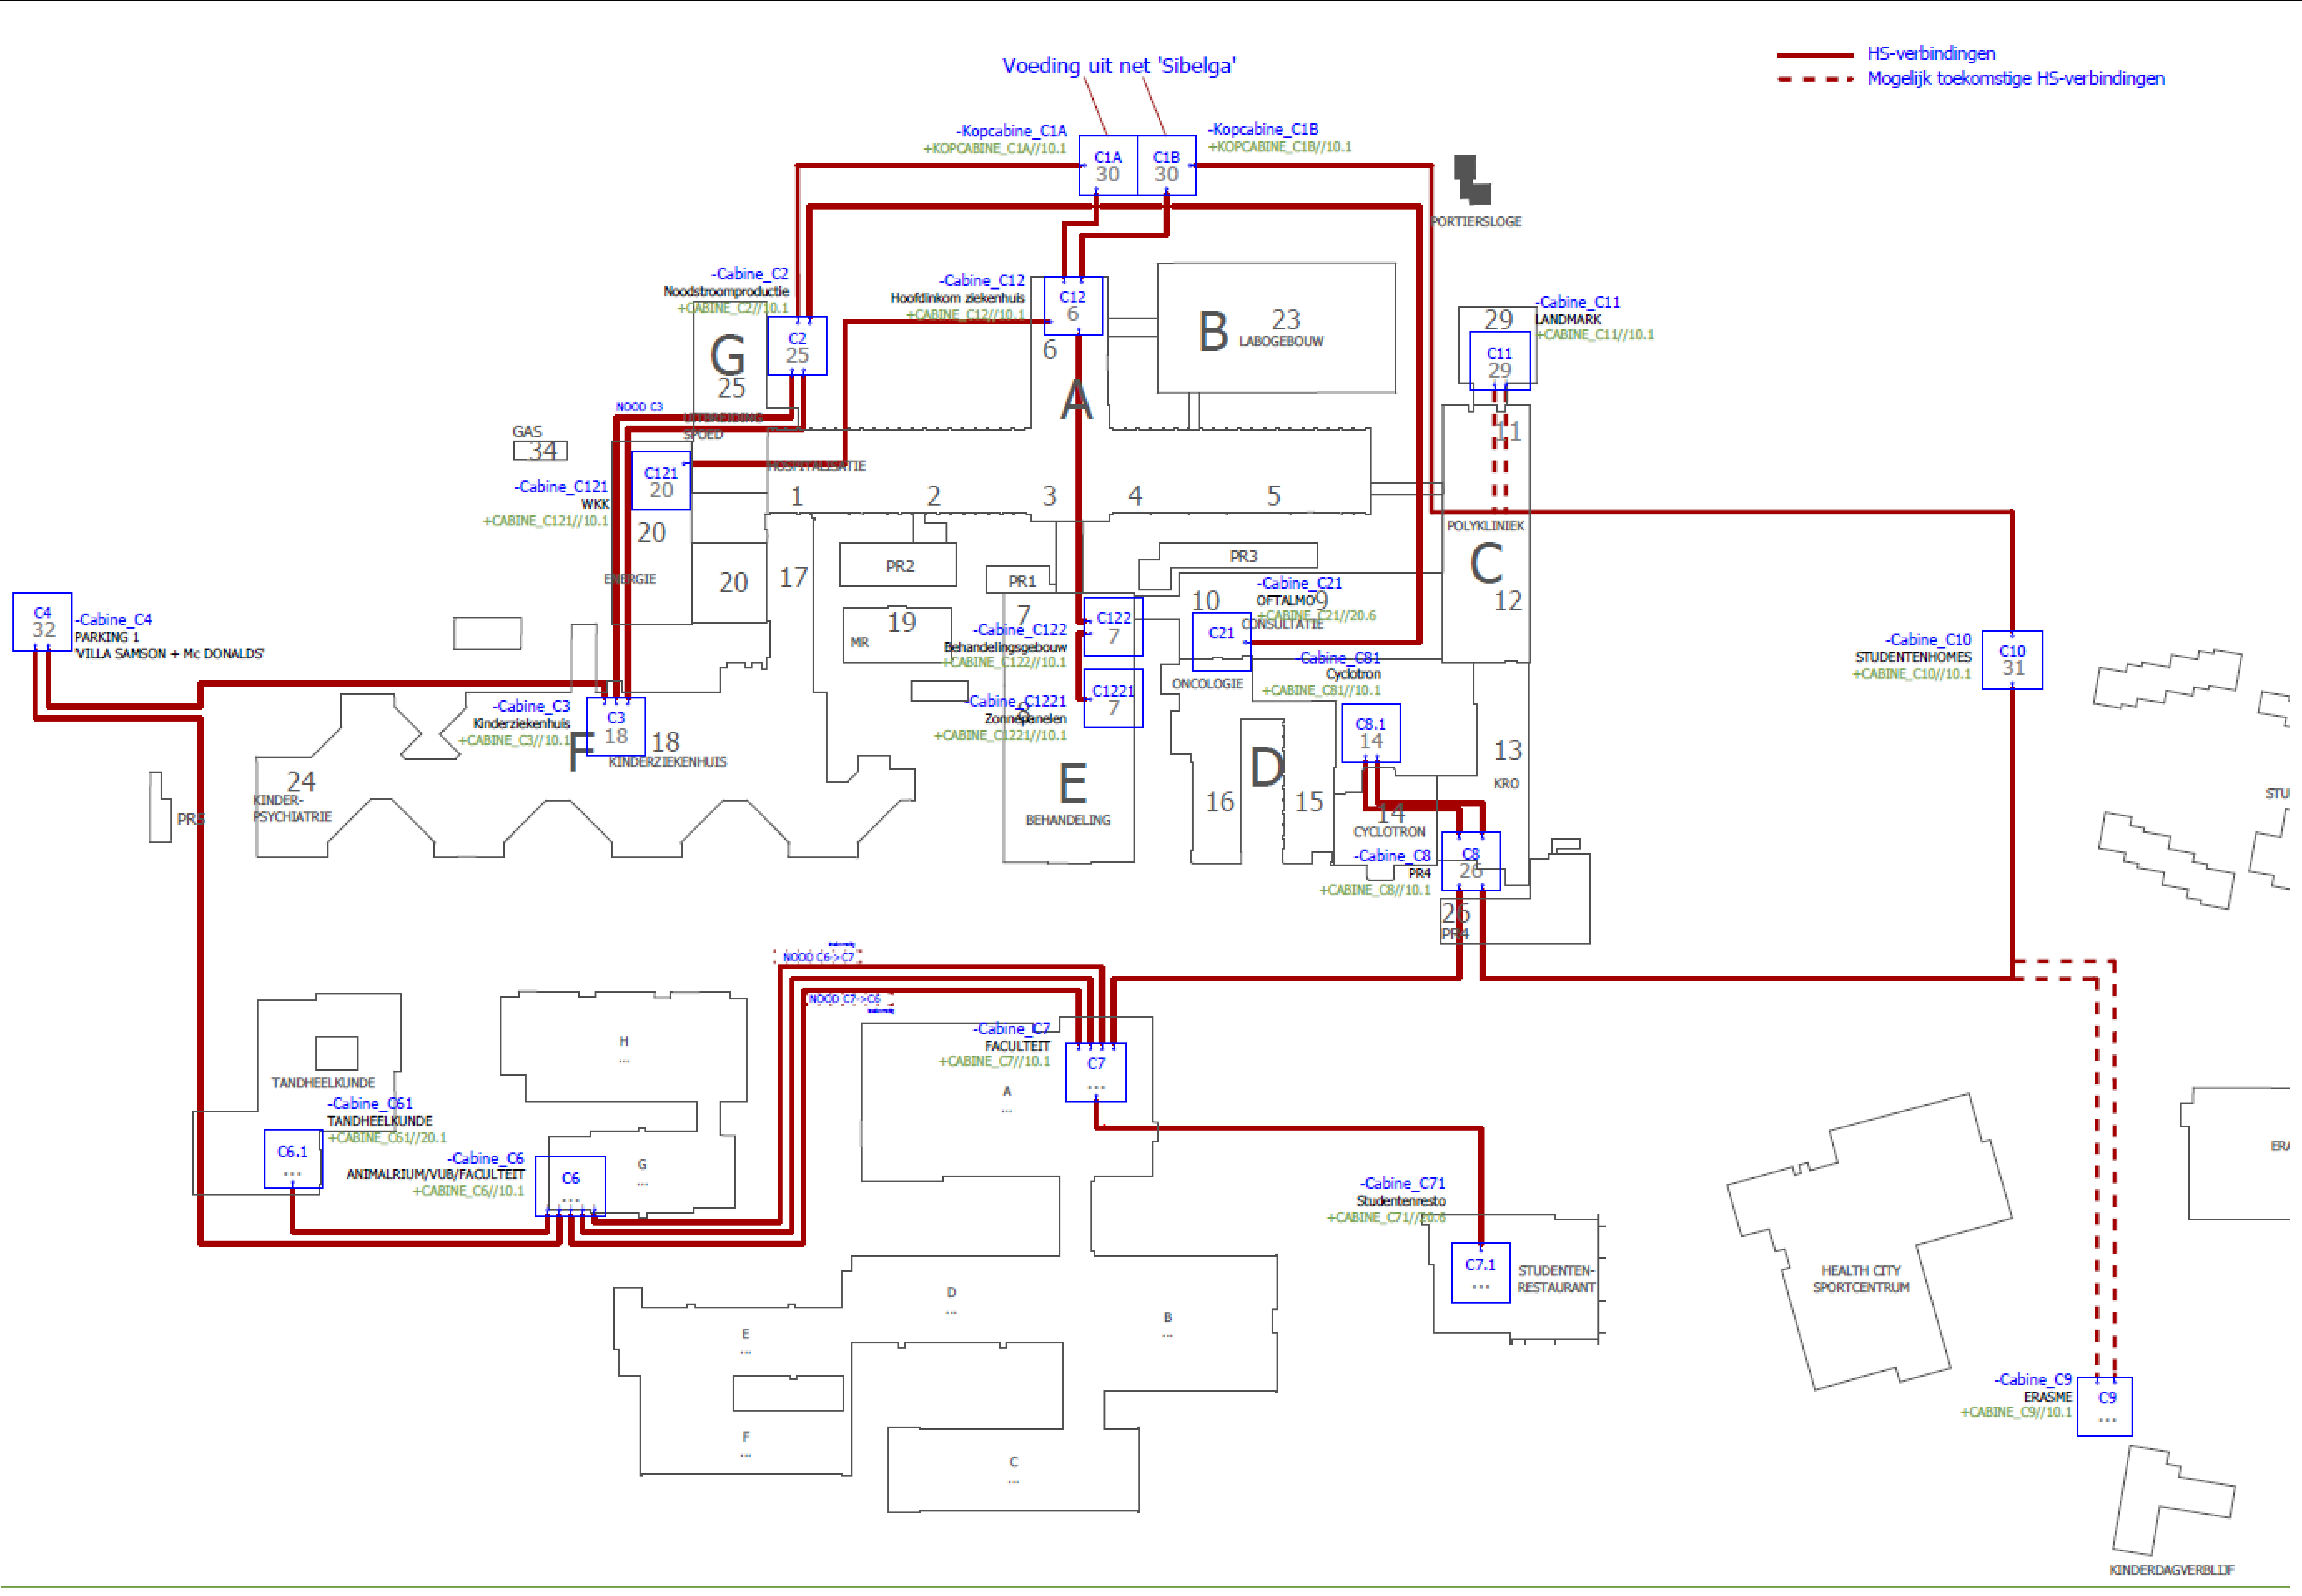
\includegraphics[width=0.97\textwidth]{vub/context/campus_site_layout.pdf}}
    \caption{\acs{UZB} electricity distribution network layout}
    \label{fig:bhc_site_layout}
\end{figure}
As part of this project the \ac{BHC}, containing the academic hospital, is a well-advanced
energy island owning and running a state-of-the-art micro-grid that can work in island mode for five consecutive days.
It includes a thermal and electricity grid, wastewater recovery, a high-speed glass-fibre telecom network and a total of 33 \ac{HV} transformers divided among 18 \ac{HV} substations.
Energy production and storage includes solar PV, \ac{CHP}, three emergency diesel generators,
and a total capacity of 2,5 MWh in battery storage, mainly under the form of UPS.
The micro-grid serves the hospital complex, 250 student dwellings, the faculty of health \& sciences, a primary school and a fitness centre. 
The micro-grid system is conceived to go in island mode with complete automatic transition in maximum 15 seconds in case of critical need and in three minute to comfort need. 
Cutting edge control technology and maximal reliability are the focus points of this demonstration site.

\begin{wrapfigure}{l}{.25\textwidth}
    \centering
    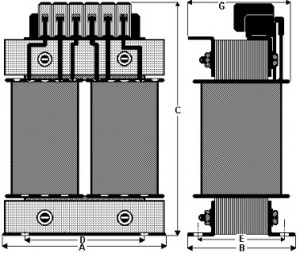
\includegraphics[width=.25\textwidth]{vub/context/trasformatori-uso-sopedaliero-300x253.jpg}
    % \caption{Example of an hospital transformer}
    % \label{fig:transformer_example}
\end{wrapfigure}
The hospital in Jette, our \textbf{main focus}, has its own distribution network, as shown in Figure \ref{fig:bhc_site_layout}.
The network's topology presents a closed-ring shape for increased reliability and is connected to the micro-grid, previously mentioned,  
through two links to nodes C1A and C1B, located at the same place. Each ``node'' of the network is \ac{HV} cabin identified by a code \{C1, C2, \dots, C12\}, with a main transformer.
Furthermore, this cabin can also have connections with one or more ``sub'' transformers, like the one here on the left, 
which are connected to ``consumers'' and/or power sources. The consumers can vary from an individual room to a whole medical department.
% or substations

\subsection{Goal(s), purpose \& critical factors}

% \todo{EB: aggiungere frasetta: ``In this section, we illustrate the company's goals'' o qualcosa del genere. Altrimenti non si capisce.}
The project started at end of July 2020, but data was collected since the 2016/17. 
So, knowing that considerable progress had already been made, I still had the added pleasure of contributing to the project in its advanced stages.
Let's see what the project's goals are in the long and short term.

\paragraph{Long term}
\begin{itemize}
    \item[$\circledcirc$] To grow Zensor into the main data hub for the Green Energy Park.
    \item[$\circledcirc$] Minimizing the energy losses and overall consumption, leading to a more profitable operation.
    \item[$\circledcirc$] To identify where the exact sources of this cost are and where the best opportunities for improvement lie.
\end{itemize}

\paragraph{Short term}
\begin{itemize}
    \item[$\circledcirc$] Having a view on the data, centralized and well accessible for multiple people in a structured way.
    \item[$\circledcirc$] Monitoring and tracking energy usage in a production site resulting in more than mere energy bill reductions.
    \item[$\circledcirc$] To improve sustainability reducing energy need and peek request. 
\end{itemize}

\subsection{Project description by phases}
\begin{figure}[ht]
    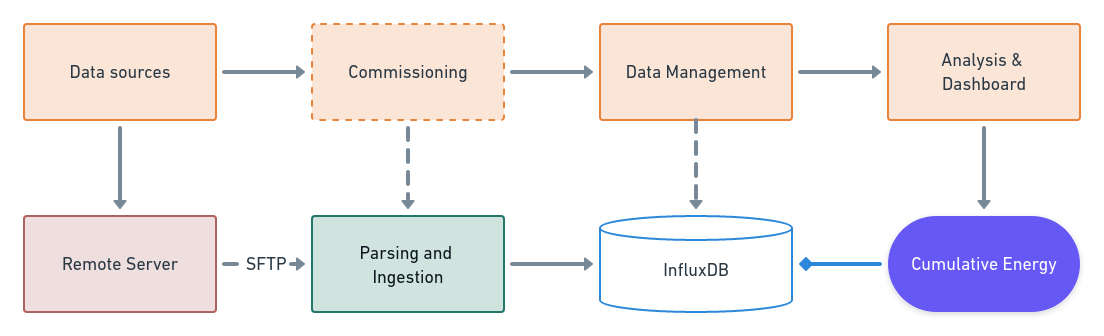
\includegraphics[width=\textwidth]{vub/flowcharts/4_phases.png}
    \caption{\ac{VUB}'s (light) project core stages}
    \label{fig:vub_stages}
\end{figure}
As we have said a few times in the previous section, see Table \ref{tab:phase_diff}, we can have two kinds of projects, full and light. 
This \ac{VUB} project falls into the lightweight class with a ``lighter'' workload, as shown in Figure~\ref{fig:vub_stages}, since the installation and engineering phase are missing. 
Data is provided by the client pre-packaged, saving a considerable amount of time needed for data-collection, but as a downside we have less control over its consistency and quality.
% \todo{EB: non capisco Inglese next ``but there with less control over its consistency and quality'' mi pare manchi un verbo}
On this project, I was primarily involved in the data engineering and analysis aspects, while keeping an eye on the context, introduced earlier, which turned out to be crucial for a successful outcome.

% All the 'items' at that point should also have a link to the manual, spec-sheet... of the component (link to Snipe-It or other database).
\paragraph{Datasources}
MOBI, one of \ac{VUB} research group, has collected through the years several MB of 15-minute data energy-related out of \ac{UZB}'s distribution network.
This limited dataset is currently stored on a remote server in a simple, yet effective way: 
a folder tree, that tries to reflect reality, and it will be our main metadata's source. 

\begin{figure}[ht]
    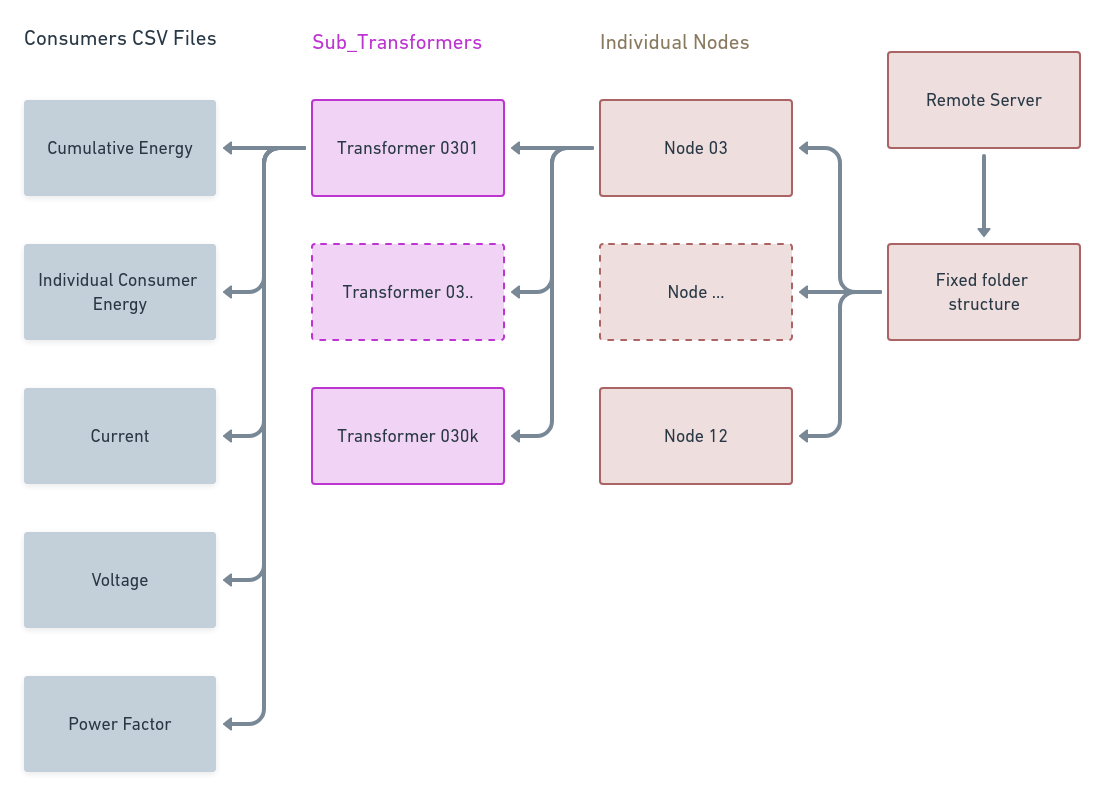
\includegraphics[width=\textwidth]{vub/flowcharts/folder_tree.png}
    \caption{\ac{VUB}'s folder tree structure}
    \label{fig:vub_folder_tree}
\end{figure}
Looking at Figure \ref{fig:vub_folder_tree} from right to left, in a bottom-up manner, should help us clarify the situation. %magari aggiungere colori ai nomi dei diversi livelli come in figura
Starting from the leaves, we found the \texttt{\ac{csv} Files}. Each file shares the same common structure with two columns, \textit{time} and \textit{value}, and multiple rows chronologically sorted.
It can either contain information about a secondary transformer or a consumer/power-source as mentioned before in Section \ref{sub:vub_initial_hp}. 
To make such distinction we must rely on its filename, indicating the hardware source and/or the physical quantity measured.
For example, we could find the file \texttt{Transfo-I3.csv}, referring to transformer's 3° phase current, while file \texttt{Bord LG 03 Radiologie.csv} stores energy consumption of the radiology department.
In our dataset different electricity measurement are present \{current, voltage, power\-factor, energy\}; all taken using the secondary \ac{LV} terminals of the transformers.
How are the different physical quantities organized? 
To answer this question, we go up one level in the tree, moving to the right, stepping up to \texttt{Measurements} where we have five separated directories.

About the energy (kWh): we have to make an important distinction between \textit{individual} or \textit{cumulative}. It can either represent the consumption of one individual consumer or the whole sub transformer, 
ideally it should be the sum of all consumers connected to it.
Instead, for the others (current, voltage e power factor) data is only available at the sub transformer level, not consumer, and in smaller quantities since it was later added to the dataset. 
Let's now change the way we traverse the tree, from bottom-up to top down i.e.\ right to left.
From the root (\texttt{Fixed folder structure}), we go down to the \texttt{Individual Nodes} layer, which is self-explanatory. We find in fact a directory for each node of our distribution network, approximately 12. 
This folder contains one or more sub-folder, one for each sub-transformer connected to the same node. Going down even further to the \texttt{Sub transformer} level, same logic applies. Each sub transformer has its own metrics folders.
So that is our connection point with the above argument.
To clarify, let us take the previous example and extend it further: the \texttt{Bord LG 03 Radiologie.csv} will have the following path in a Unix-like OS: \textit{root/NodeC03/Transformer0302/ConsumerEnergy/Bord\dots}.
%So each set of voltage-files is grouped in to a folder

\paragraph{Commissioning \& Data Management}
% Spostare i dati da un server all'altro e digerirli
\begin{figure}[ht]
    \includegraphics[width=\textwidth]{vub/flowcharts/data-management.png}
    \caption{\ac{VUB}'s data ingestion flowchart}
    \label{fig:vub_ingestion}
\end{figure}
Once the university granted us the credentials to remotely access this folder, we could start to manage it by accessing it using \ac{SFTP} over port 9921. % that is periodically
The \textbf{first step} of the ingestion is, as illustrated in the Figure \ref{fig:vub_ingestion}, copying data from \ac{VUB}'s server to Zensor's one. 
This happens periodically as cron job, as mentioned in Section \ref{subsection:script_structure}, also thanks to Python library \texttt{pysftp}. %enumerate?
The script recursively traverses the sftp folder and if it comes across a .csv file, it copies it into the same folder structure as on the server.

Subsequently, for \textbf{step two}, after closing the \ac{SFTP} connection, we can work with our freshly copied data. We traverse, once again, the folder tree, keeping track of
folder names that are going to be important as metadata. Once we are at leaf level, see once again Figure \ref{fig:vub_folder_tree}, we use 
Pandas (\ref{section:pandas}) for handling file reading and inferring the date-time strings format. This switch to a faster parsing method can potentially increase the speed by 5-10x. %parsing
Then we can perform some data cleaning, for eliminating outliers, duplicates and non-numerical values out our DataFrames, one for each file.
Afterwards we tag the respective \textbf{DataFrame} with the necessary information to easily identify it, like description, unit and other metadata previously collected.

Since the files are numerous and of significant size, this series of operations can take a long time. 
Therefore, it was decided to parallelize the whole operation using a pool of processes, not threads. To substantiate this point, here is a small digression: 
in Python, if code is \textit{CPU-bound}, multithreading won't help, because only one thread can hold the Global Interpreter Lock, and therefore run Python code, at a time. 
So, in this specific scenario we need to use processes, not threads, since in multiprocessing, any newly created process will run independently with its own memory space.

Finally, the \textbf{step three} involves writing each DataFrame on the InfluxDB (\ref*{section:influxdb}), our choice for \acl{tsdb}.
This operation, which is already quite optimized, can be easily executed in parallel given the limited concurrency.
As a result, we will have a \textit{``measurement''} for each node, which will contain several series, one for each consumer, easily distinguishable from the others.

% In a second instance they want the entry point to be a map of the campus with the main transformers indicated and with a clickable link on each item such that the data can be consulted. 
\paragraph{Analysis \& Visualization}
\begin{figure}[ht]
    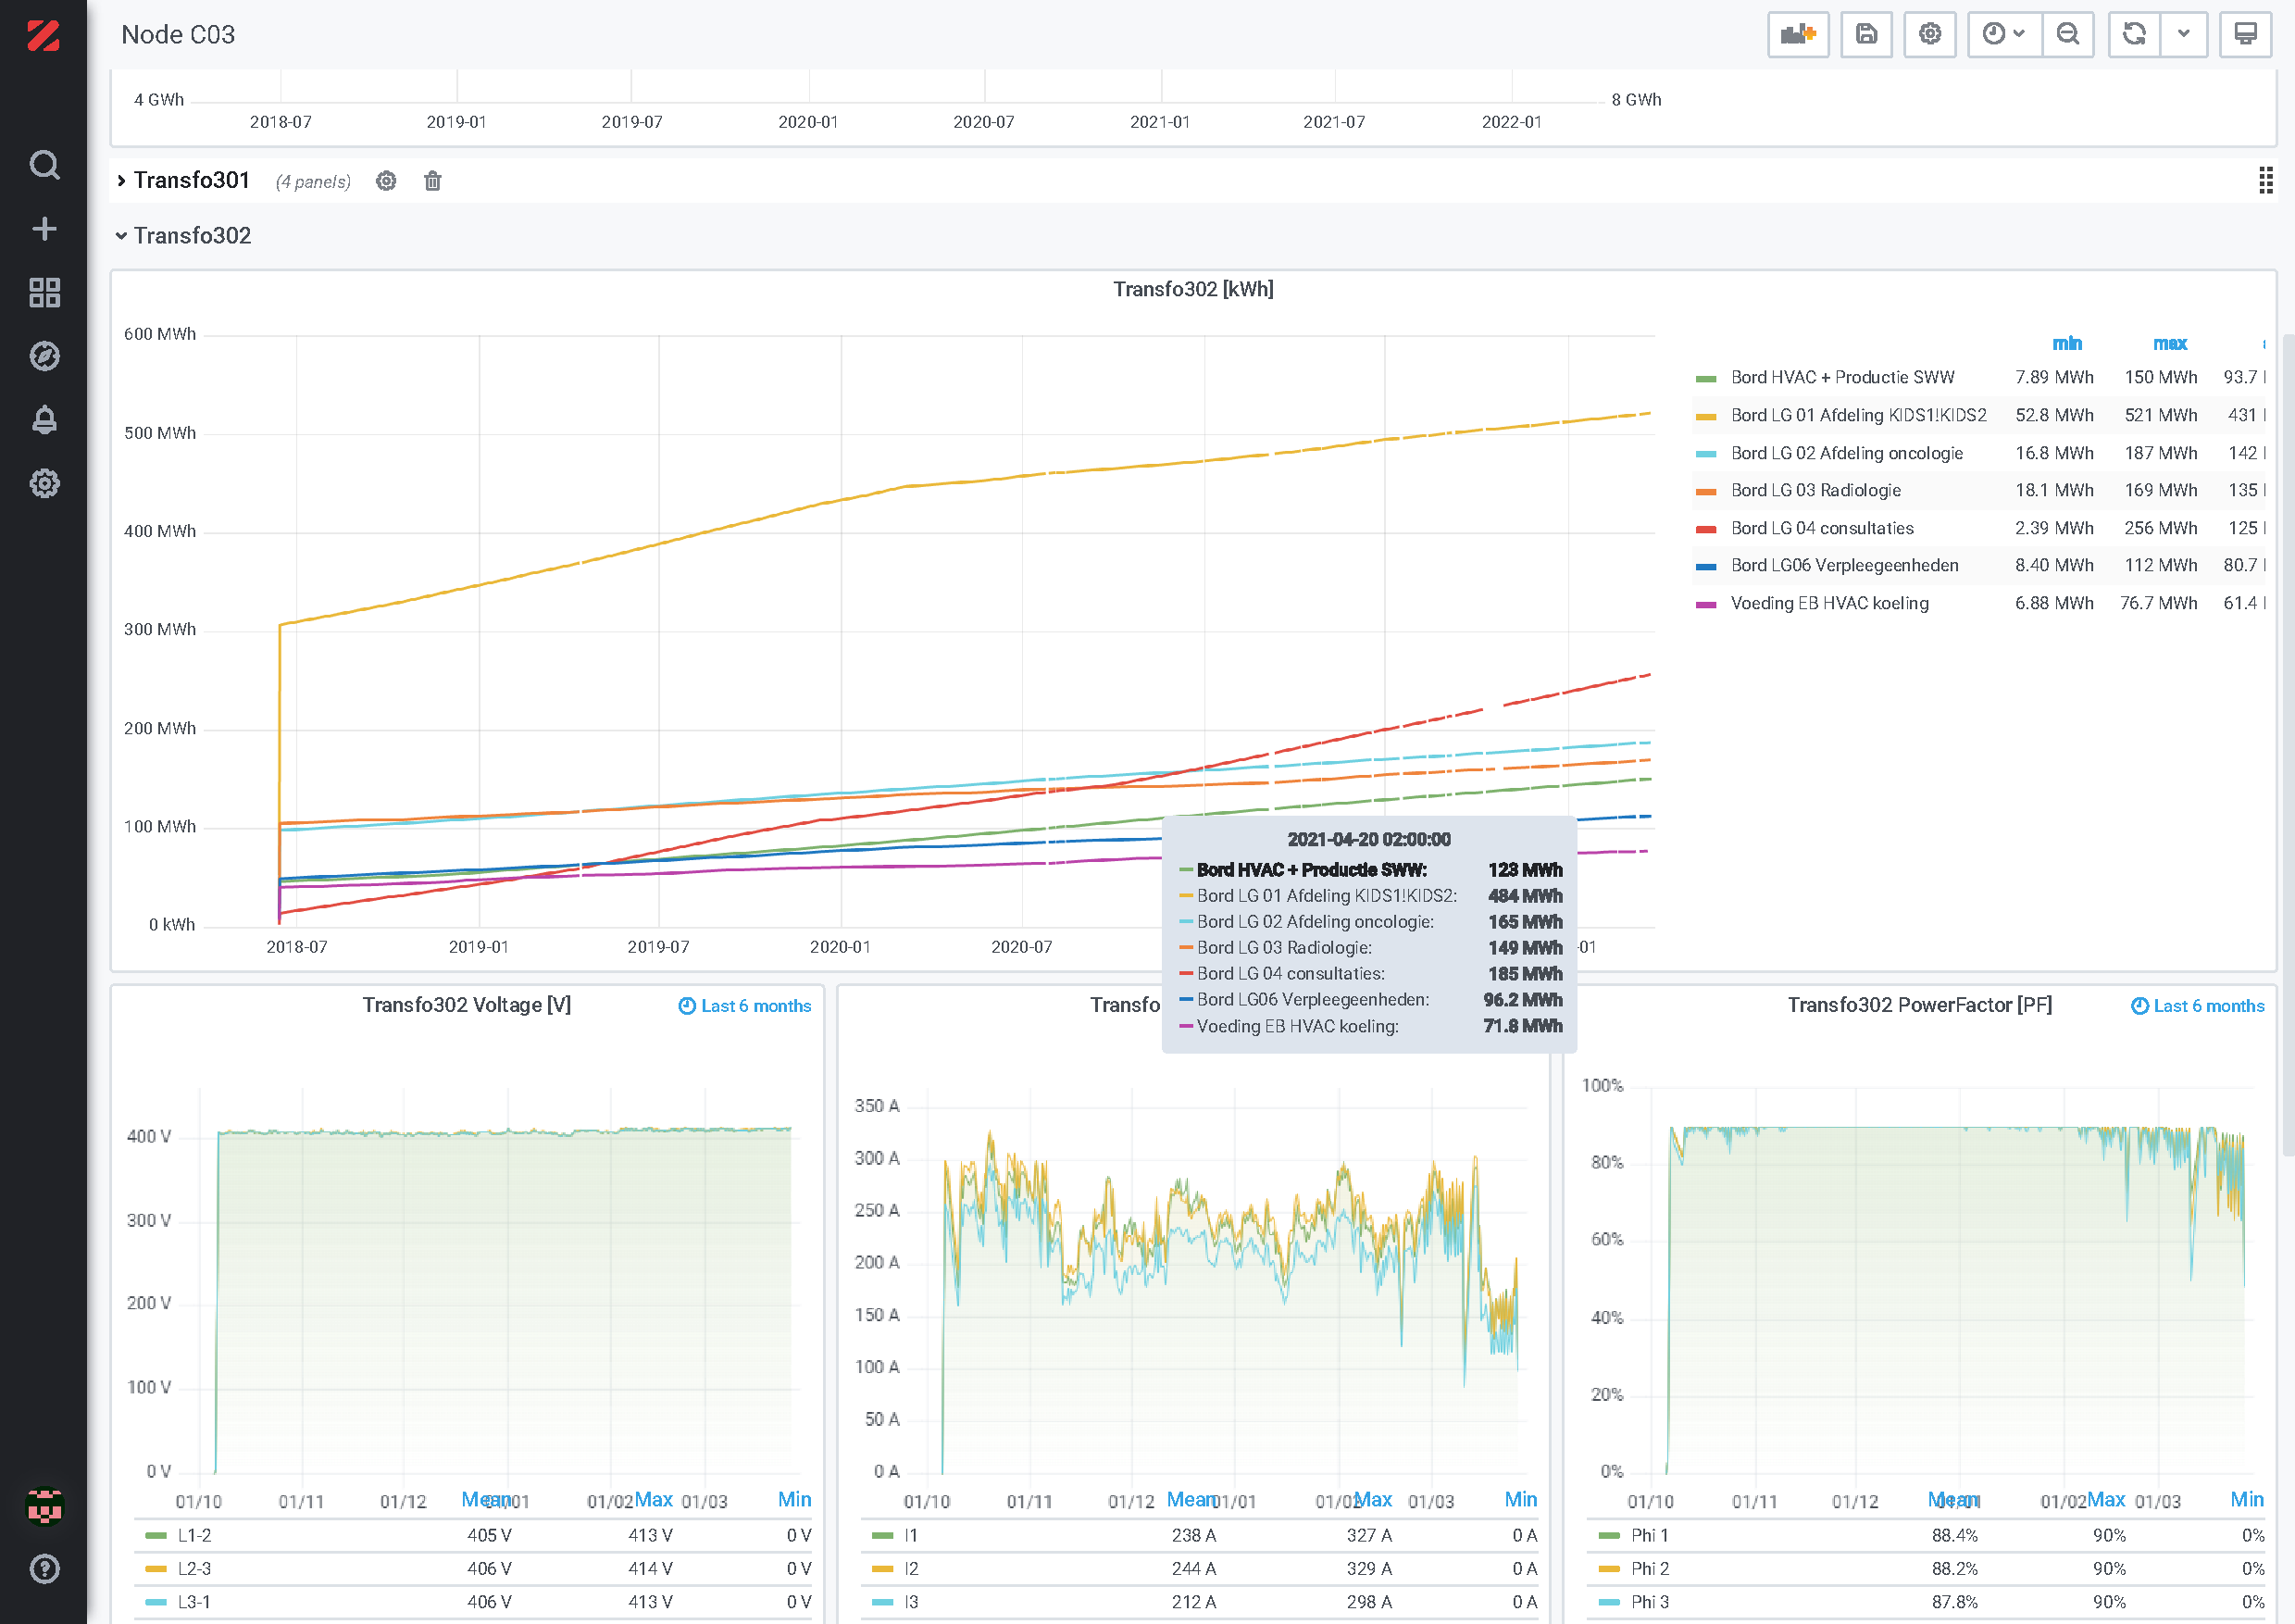
\includegraphics[clip, trim=0 0 0.1cm 3.5cm, width=\textwidth]{vub/grafana/node_c03_transfo302_raw.pdf}
    \caption{Transformer302 raw data dashboard}
    \label{fig:vub_raw_rad}
\end{figure}
To ensure that ingestion has been carried out correctly some basic visualizations is required.
Therefore, we designed the dashboards to share the same structure, same philosophy as the distribution network.
So, each node (\ac{HV} cabin) will have its own page, with a variable number of panels, depending on how many sub-transformers are present per node.
Taking the Node C3 dashboard as an example, illustrated in Figure \ref{fig:vub_raw_rad}, enhanced with a bit of contextual information: 
the station gives power to the children's hospital, as we can spot references to medical wards in the legend, and has three sub-transformers.
In particular we will focus on the second one and its metrics, where we can recognise some key elements previously discussed.
Starting from the bottom, we find three panels covering transformer's (Transformer 302) voltage, current and power factor, with a minimum six months temporal frame.
As mentioned at the beginning of this segment, these measurements were added at a later stage and are in a smaller volume than the electric energy. 
At this stage of the project, there is not a high interest in performing any analyses on these metrics, besides trend monitoring. 
Directly above, a larger panel visualises the energy consumption of all 7 consumers connected to the transformer.
As we discussed in Section \ref{section:grafana}, \textit{Grafana} allows us to adjust the time window to our liking.
In the time interval chosen, from July 2018 to March 2022, each signal appears to be a monotonously increasing function of time $f(t)$. 
In fact, corresponding data, measured at the \ac{LV} stations, is cumulative: easy to collect and store, but less interesting from an analytical point of view. 
Following this argument, we should not be surprised that, taking a random point (20 April 2021), the different energy consumption values recorded at that instant 
are of a higher order of magnitude [MWh] than expected [KWh].
% We will resume this issue at later stages.
\begin{figure}[ht]
    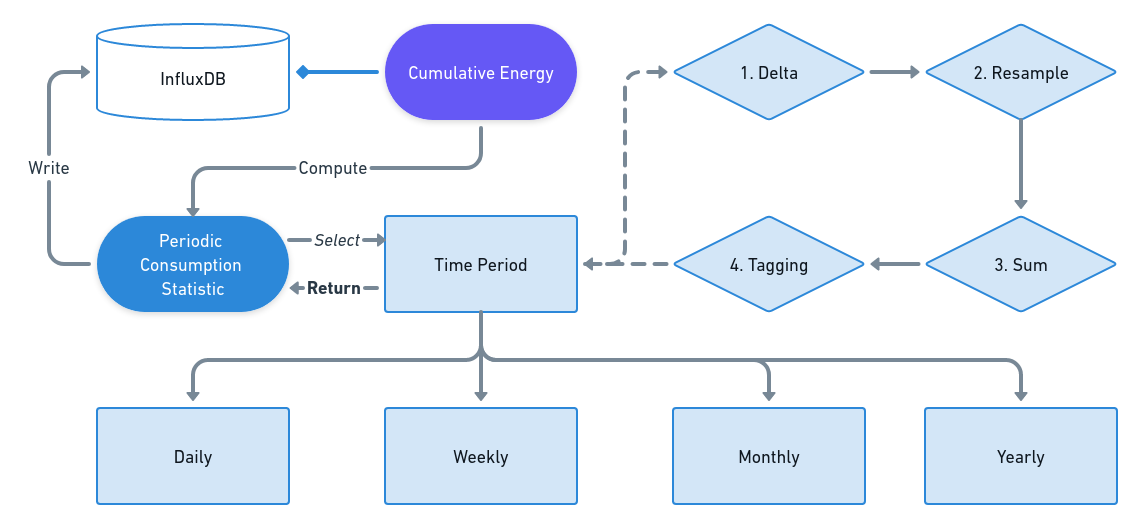
\includegraphics[width=\textwidth]{vub/flowcharts/analystic_flowchart.png}
    \caption{\ac{VUB}'s analytics chart}
    \label{fig:vub_anal_chart}
\end{figure}

One of the objectives of this project is to provide information on the energy intake of the various nodes, making more effective use of these data. 
The next step is then to calculate appropriate usage statistics, also to answer common questions such as: what is the average consumption of transformer $x$?
We now shall examine the workflow of operations necessary for achieving this goal.
Looking at the diagram in Figure \ref{fig:vub_anal_chart}, we can observe that the first necessary step is to choose a time period $T$, daily to yearly.
Ideally, for the end user i.e.\ the VUB researcher, all options will be available, but certainly the daily $T$ is highly informative.
As for the subsequent steps, they are quite intuitive at an abstract level.
\begin{enumerate}
    \item First, following the previous discussion, we calculate how much the series varies. 
    That is, taking two successful points of the signal $x_t$ and $x_{t+1}$ we calculate the delta i.e.\ $\Delta = x_{t+1} - x_t$.
    \item Second, using pandas split-apply-combine approach, as discussed in Figure \ref{fig:pandas_groupby}, we group on our tag columns; then we use the library downsampling 
    functionality for performing a frequency conversion on $\Delta$-data: from 15-minutes to the selected $T$ period.
    \item Third, we compute the group sum, as the apply step and we get our data combined as requested.
    \item Four, we tag the resulting DataFrame with extra information, such as the resulting frequency, quite useful for visualization and querying purposes.
\end{enumerate}

So, all that remains is to visualise the \textit{periodic consumption} statistic in an intelligent way, providing some insights for researchers.
We shall now take a look at two dashboards, illustrated in Figure \ref{fig:vub_2_dashboard}, with several panels using a range of visualisation techniques, but querying the same statistic.
As mentioned in the figure's caption, we are displaying data concerning the preceding case, i.e. the radiology department of the children's hospital.
In detail, starting from dashboard (\subref{fig:vub_stats_v1}), we find, on the top left corner, a panel representing the daily consumption distribution, which is mainly between 20 and 80 kWh. 
On the right side we can see, instead, a pie chart about the proportional average intake per day of the week, where the maximum is Tuesday and the minimum Sunday. 
Finally, at the bottom, we have a status map which gives us, at one glance, a comprehensive view of long-term average daily consumption. 
For instance, we were able to notice that on 28th December 2022 there was a spike in usage, with a value of 235 kWh.

Turning now to Figure (\subref{fig:vub_stats_v2}), we can see that it consists of 3 panels. Starting again from the top left-hand corner, 
we have a bar plot, indicating the average energy consumption per day of the week. % averaged over the selected period. 
Note that the y-axis does not start from 0, but from 37.5 to highlight the present differences. 
On the right, we find once again a pie chart, similar representation to that discussed for panel (\subref{fig:vub_stats_v1}).
Finally, at the bottom we see another bar plot, horizontally aligned, visualising the same daily average over a longer period, i.e. a month, with peaks in June and July and lows in October. 
As a minor distinction between the two is that (\subref{fig:vub_stats_v1}) have transparent panels, as contrasting with the white background of (\subref{fig:vub_stats_v2}). 
With these considerations,  we can consider close the discussion, knowing that a few aspects have been left out, to keep the text as relevant and clean as possible.
% \todo{EB: meglio ``we can close the discussion'' o simili?}

\begin{figure}
    \begin{subfigure}{\textwidth}
        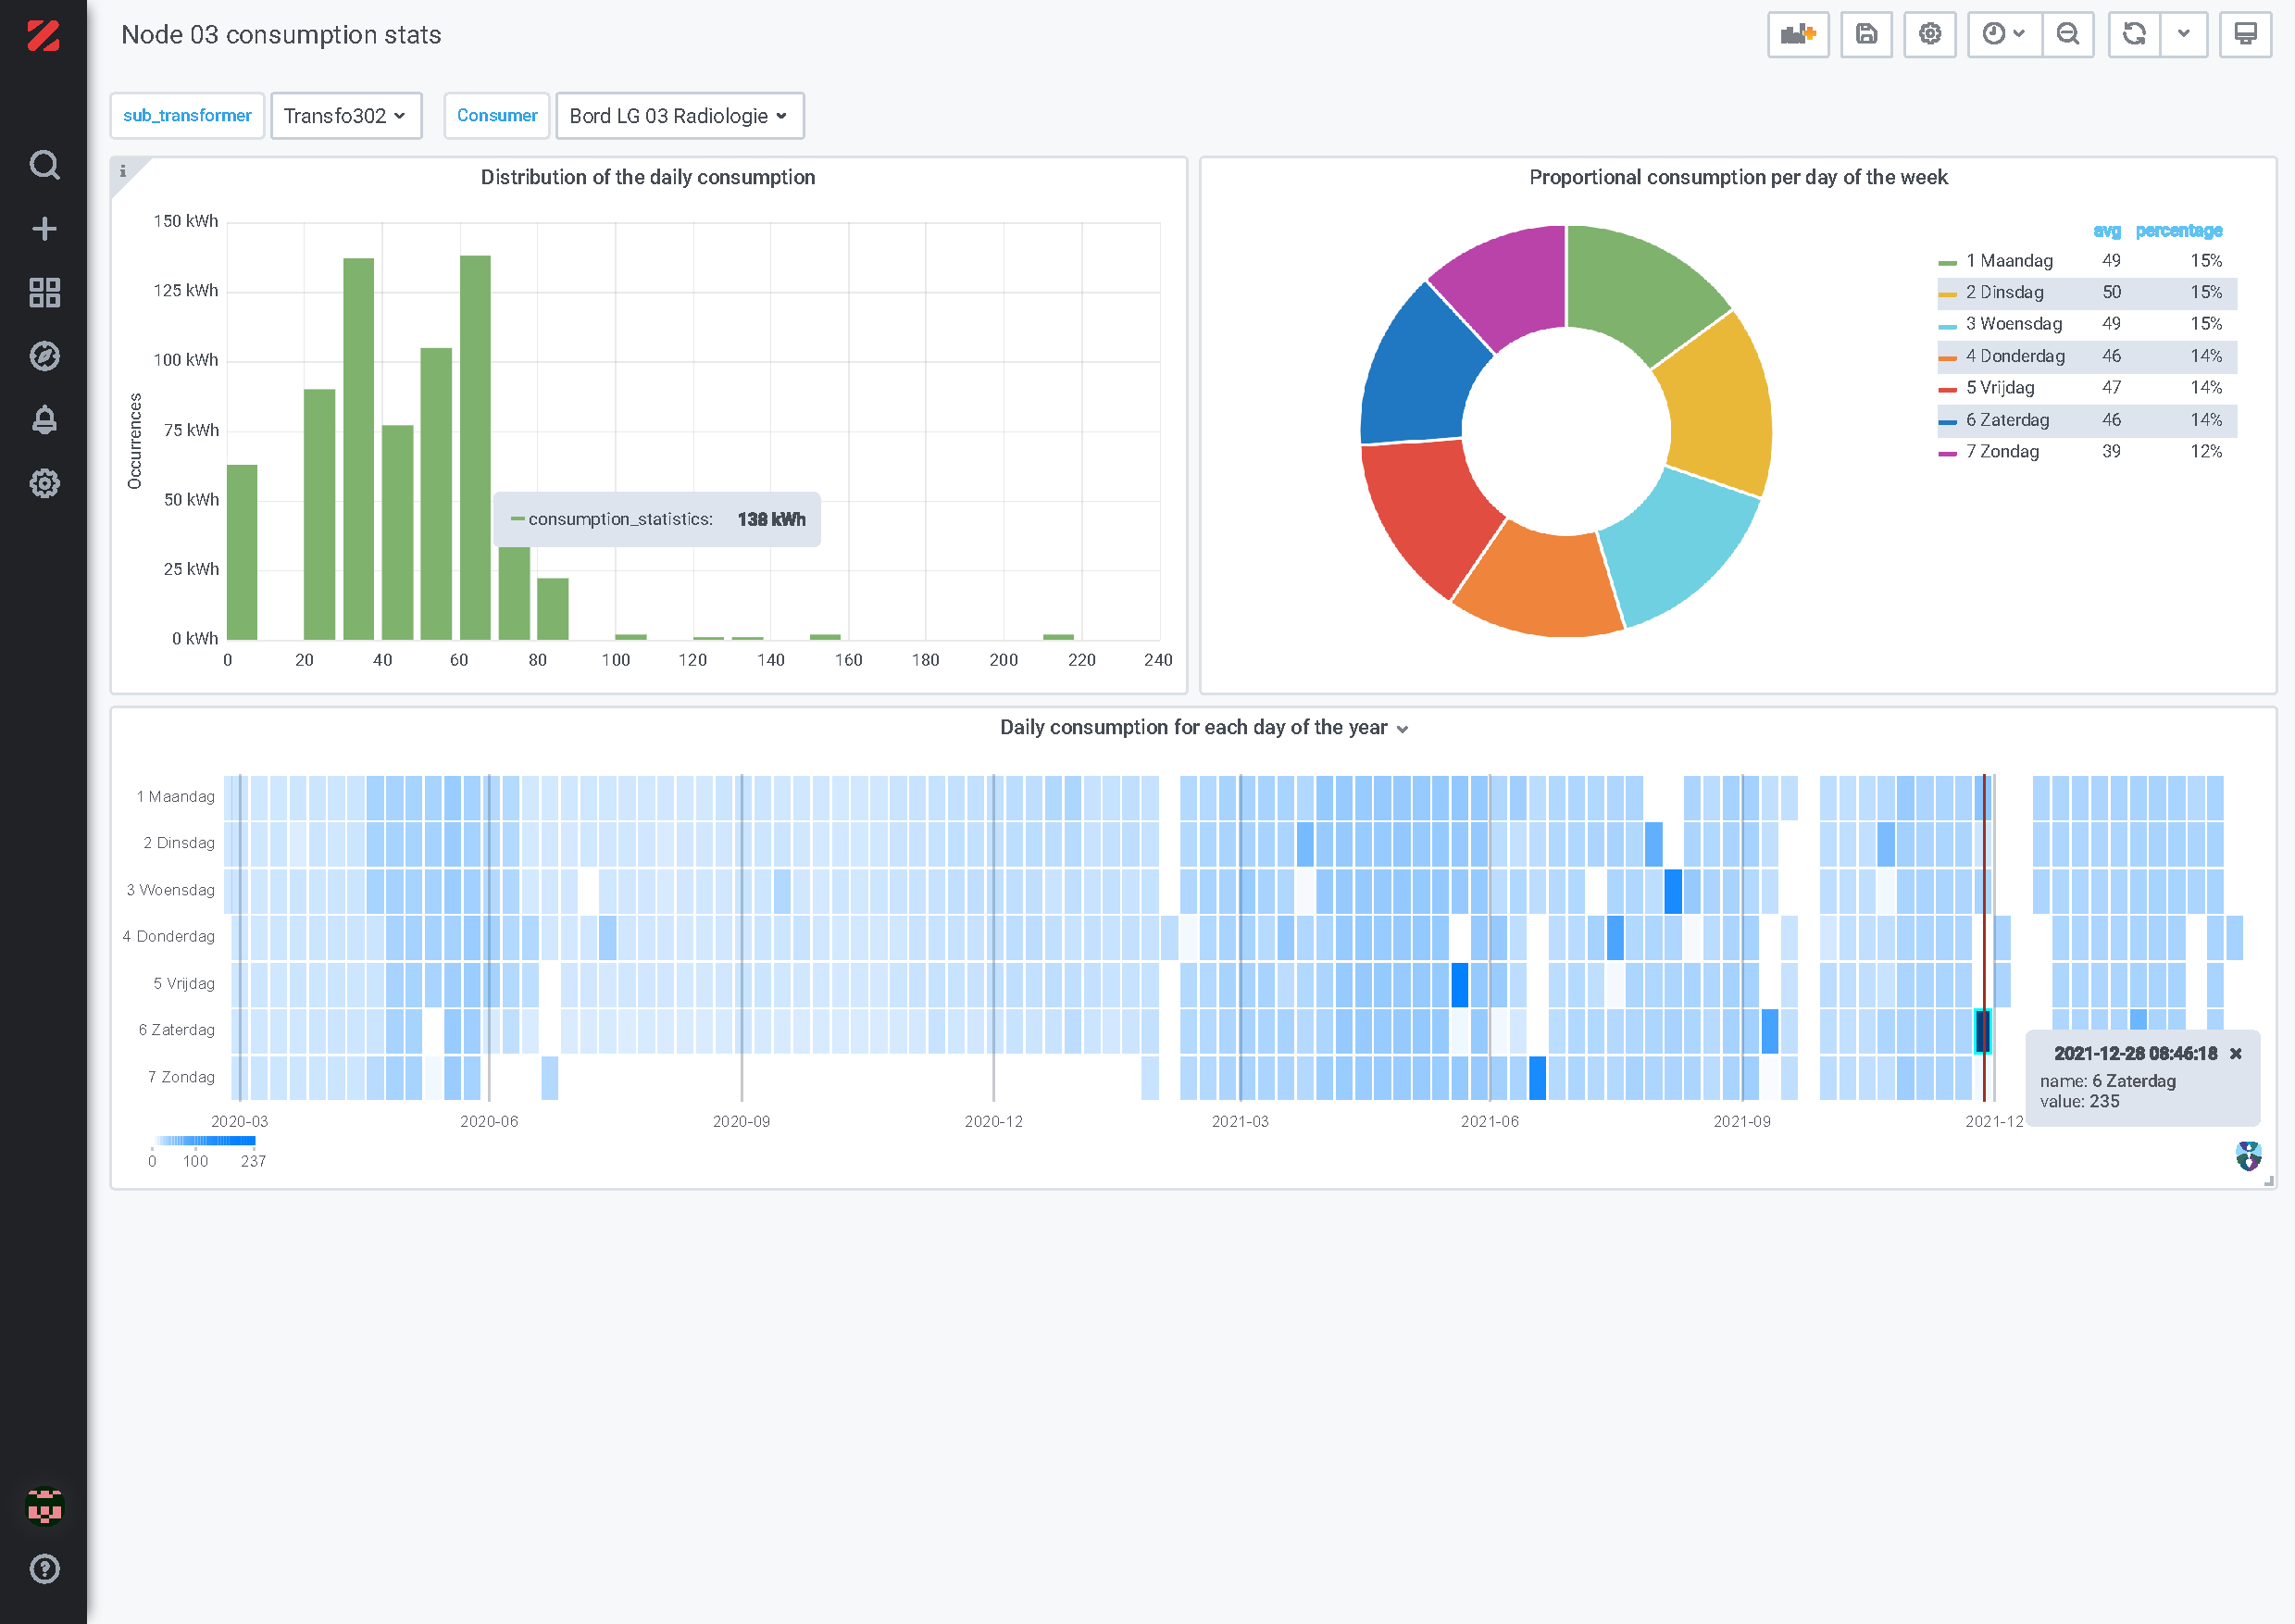
\includegraphics[clip, trim=0 7.5cm 0 0, width=\textwidth]{vub/grafana/node_c03_consumption_stats.pdf}
        \caption{Daily distribution}
        \label{fig:vub_stats_v1}
    \end{subfigure}
    \begin{subfigure}{\textwidth}
        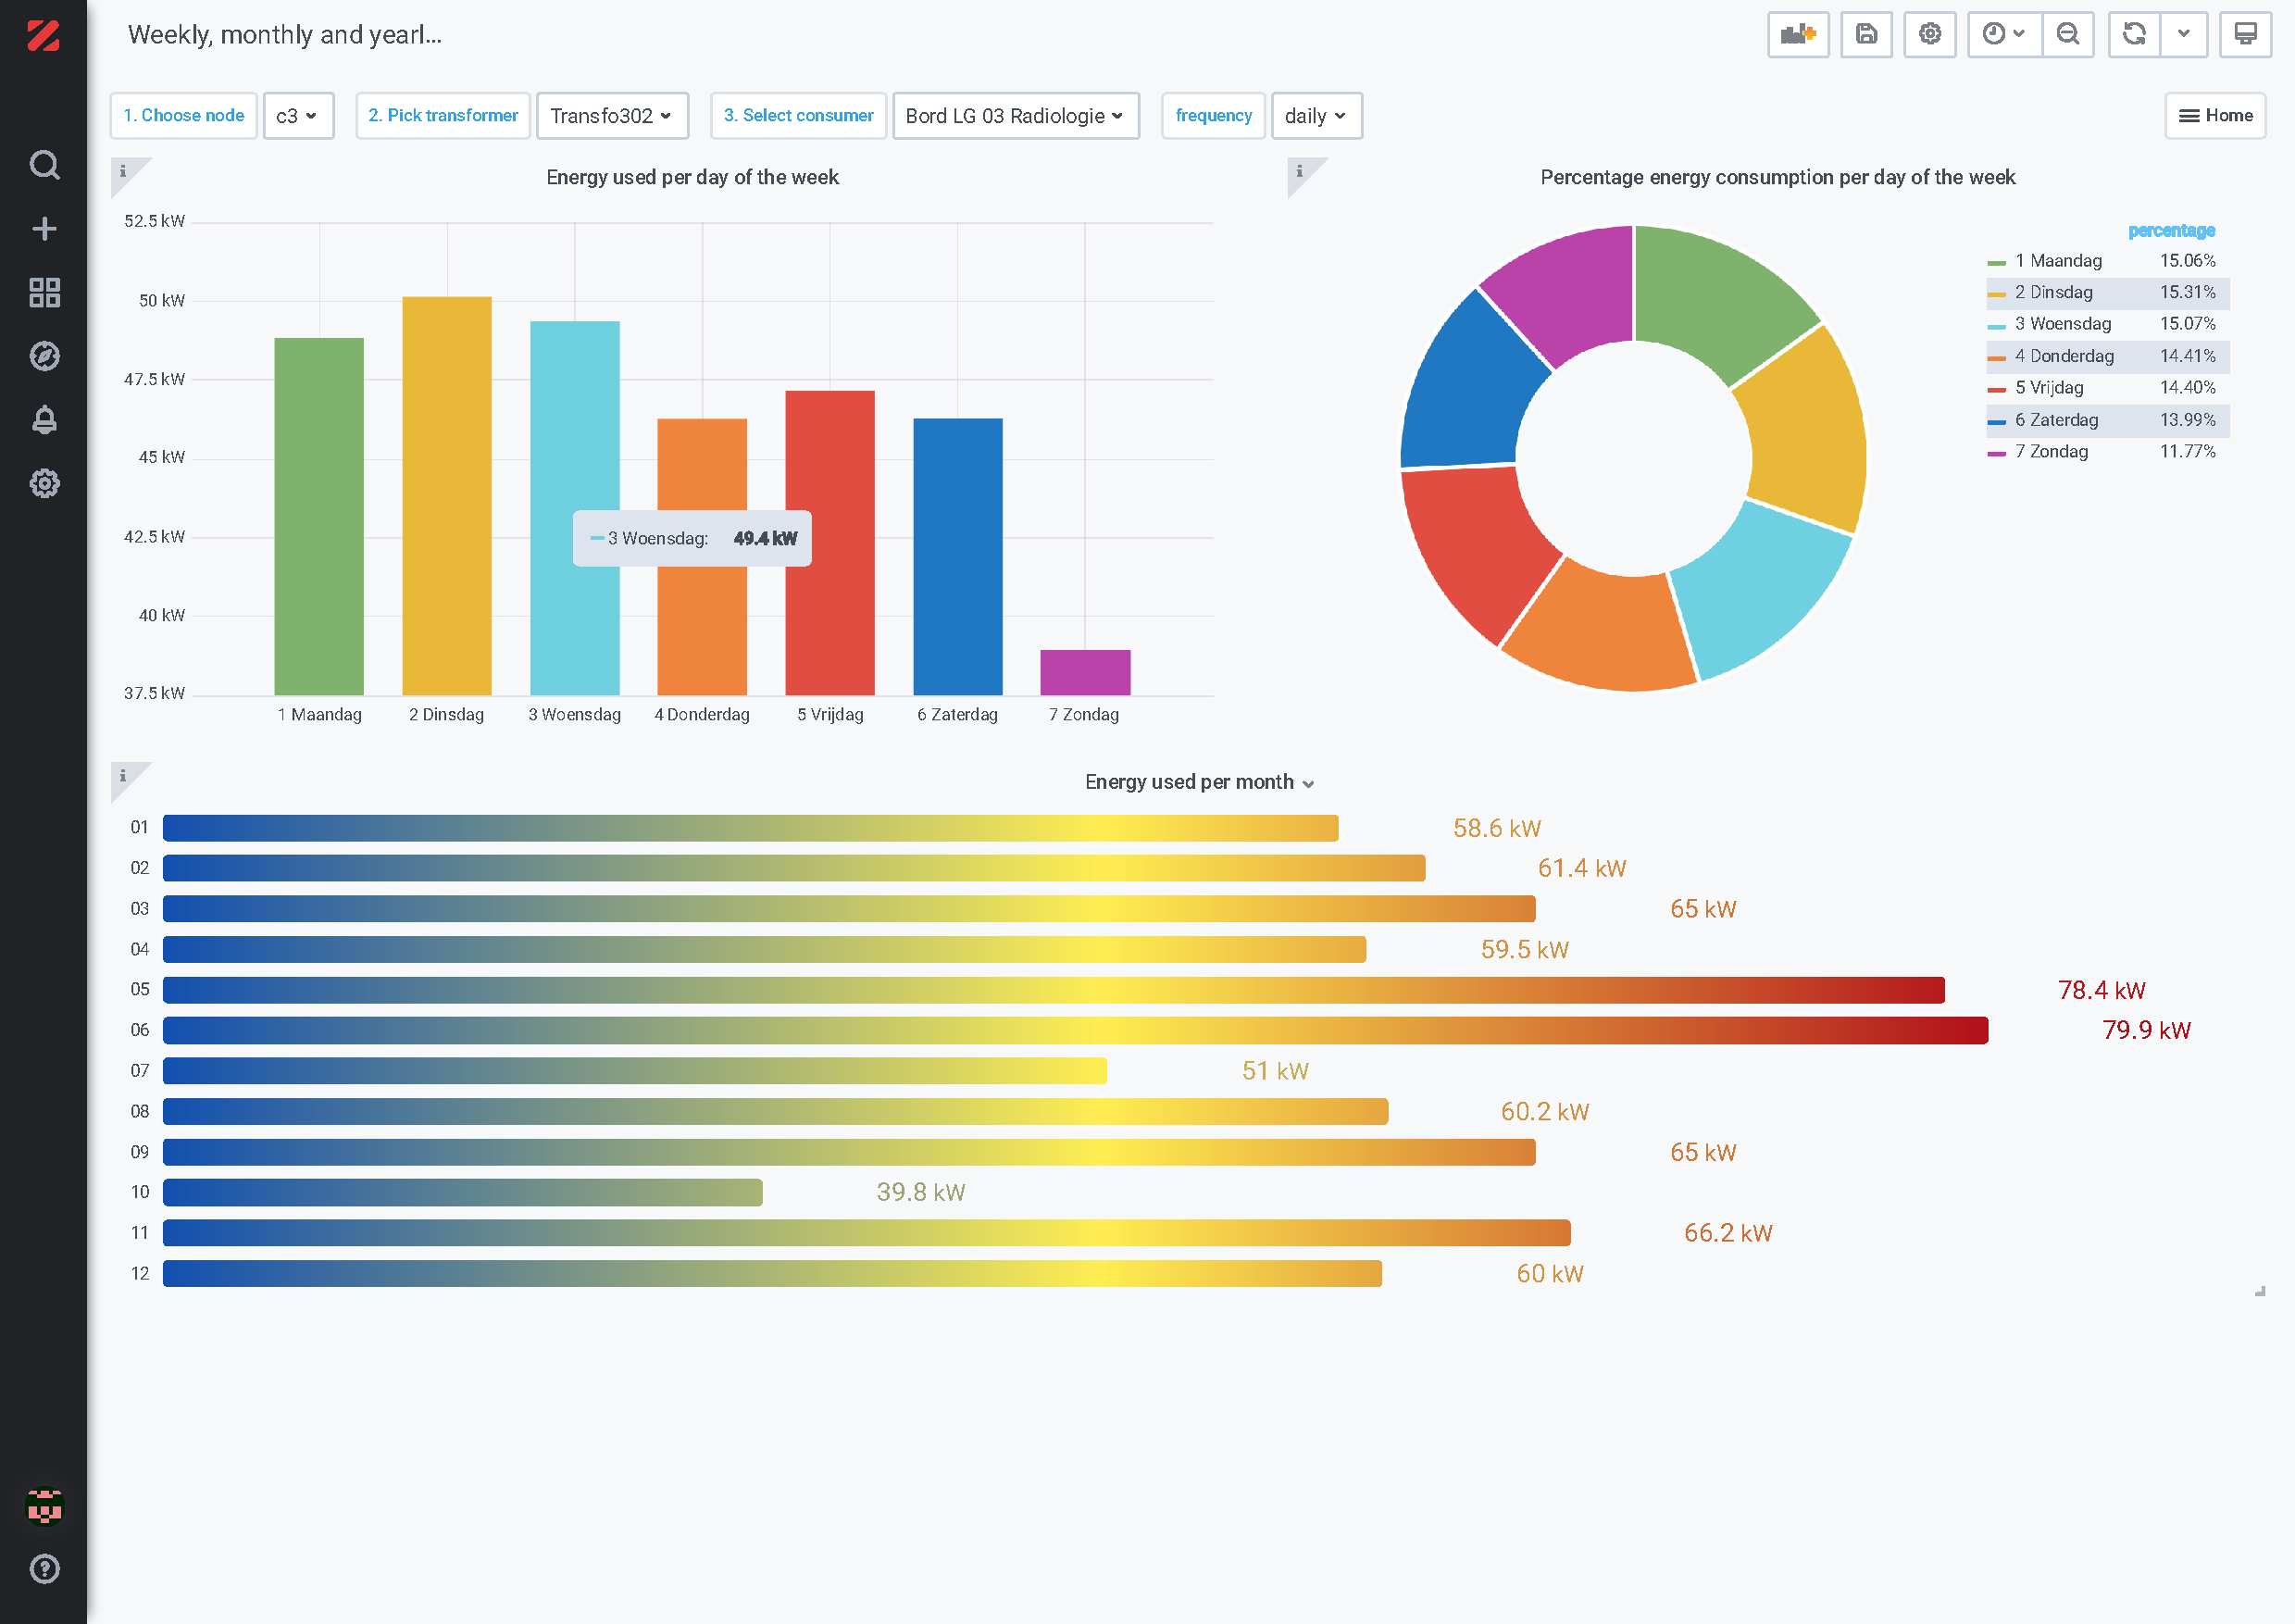
\includegraphics[clip, trim=0 5.5cm 0 0, width=\textwidth]{vub/grafana/weekly_and_monthly_node_c3_transfo302_radio.pdf}
        \caption{Per day of the week \& month}
        \label{fig:vub_stats_v2}
    \end{subfigure}
    \caption{Two examples of visualization dashboard of \ac{UZB} radiology's energy consumption}
    \label{fig:vub_2_dashboard}
\end{figure}

\subsection{Conclusion}
Concluding, we can state that \ac{VUB} researchers were fairly satisfied with the project result, as they now are able to monitor most of the hospital consumption via dashboards, in detail, everywhere through a web browser.
As evidence of this, they also decided to further expand the plan by adding a considerable amount of \ac{GEP} data, which became a separate sub-project.
% sextant \todo{EB: sicuro del ``sextant''?} No ho preso una cantonata.
However, potential enhancements remain open, such as additional statistics to compare nodes and viable alarms on current, voltage and power factor values. 


